\subsection{Упражнение 1}

Запустите и прослушайте примеры в файле chap03.ipynb. В примере с утечкой попробуйте заменить окно Хэмминга одним из других окон, предоставляемых NumPy, и посмотрите, как они влияют на утечку.

\begin{lstlisting}[language=Python]
signal = SinSignal(freq=440)
duration = signal.period * 30.25
wave = signal.make_wave(duration)
spectrum = wave.make_spectrum()
spectrum.plot(high=880)
\end{lstlisting}

\begin{figure}[H]
	\begin{center}
		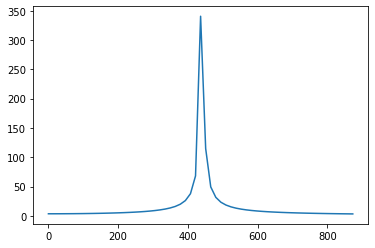
\includegraphics[scale=1]{fig/lab03/lab03_4_0.png}
		\caption{Рассматриваемый сигнал}
	\end{center}
\end{figure}

Посмотрим как выглядит спектограмма с использованием окна Хэмминга:

\begin{figure}[H]
	\begin{center}
		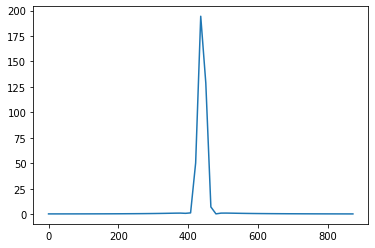
\includegraphics[scale=1]{fig/lab03/lab03_6_0.png}
		\caption{Сигнал с использованием окна Хэмминга}
	\end{center}
\end{figure}

Посмотрим остальные окна


Окно Бартлетта:
\begin{lstlisting}[language=Python]
wave = signal.make_wave(duration)
wave.ys *= np.bartlett(len(wave.ys))
spectrum = wave.make_spectrum()
spectrum.plot(high=880)
\end{lstlisting}
\begin{figure}[H]
	\begin{center}
		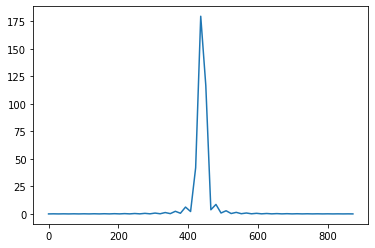
\includegraphics[scale=1]{fig/lab03/lab03_9_0.png}
		\caption{Сигнал с использованием окна Барлетта}
	\end{center}
\end{figure}
Можно заметить. что низкие амплитуды стали ломанными линиями.


Окно Блэкмена:
\begin{lstlisting}[language=Python]
wave = signal.make_wave(duration)
wave.ys *= np.blackman(len(wave.ys))
spectrum = wave.make_spectrum()
spectrum.plot(high=880)
\end{lstlisting}
\begin{figure}[H]
	\begin{center}
		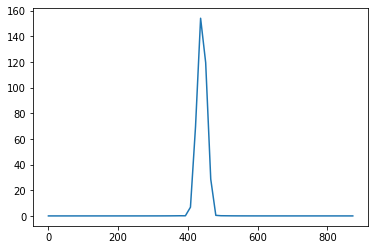
\includegraphics[scale=1]{fig/lab03/lab03_12_0.png}
		\caption{Сигнал с использованием окна Блэкмена}
	\end{center}
\end{figure}

Видим. что утечка стала линейно переходить к нужной частоте.

Окно Хэннинга:
\begin{lstlisting}[language=Python]
wave = signal.make_wave(duration)
wave.ys *= np.hanning(len(wave.ys))
spectrum = wave.make_spectrum()
spectrum.plot(high=880)
\end{lstlisting}
\begin{figure}[H]
	\begin{center}
		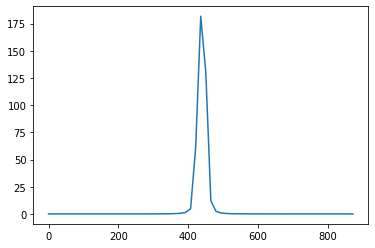
\includegraphics[scale=1]{fig/lab03/lab03_15_0.png}
		\caption{Сигнал с использованием окна Хэннинга}
	\end{center}
\end{figure}

Все четыре хорошо справляются с уменьшением утечек. Фильтр Бартлетта имеет небольшой шум на переходе. Фильтр Хэмминга рассеивает наименьшее количество энергии.
\subsection{Упражнение 2}


Напишите класс SawtoothChirp, расширяющий Chirp и переопределяющий evaluate для генерации пилообразного сигнала с линейно увеличивающейся частотой.

\noindent Нарисуйте эскиз спектограммы этого сигнала, затем распечатайте её. Эффект биение должен быть очевиден, а если сигнал внимательно прослушать, то биения можно и услышать.

\begin{lstlisting}[language=Python]
class SawtoothChirp(Chirp):

    def evaluate(self, ts):
        
        freqs = np.linspace(self.start, self.end, len(ts))
        dts = np.diff(ts, prepend=0)
        dphis = 2 * np.pi * freqs * dts
        phases = np.cumsum(dphis)
        cycles = phases / (2 * np.pi)
        frac, _ = np.modf(cycles)
        ys =  normalize(unbias(frac), self.amp)
        return ys
\end{lstlisting}

Создадим звук:

\begin{lstlisting}[language=Python]
signal = SawtoothChirp(start = 440, end = 880)
wave = signal.make_wave(duration=1, framerate=4000)
wave.make_audio()
\end{lstlisting}

Слышно, как частота постепенно увеливается.

Выполним кратковременное преобразование Фурье и представим результат в виде спектограммы. По оси OY будет частота, по оси OX время.

\begin{lstlisting}[language=Python]
sp = wave.make_spectrogram(256)
sp.plot()
\end{lstlisting}
\begin{figure}[H]
	\begin{center}
		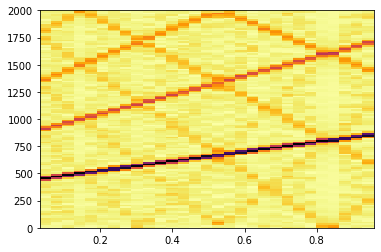
\includegraphics[scale=1]{fig/lab03/lab03_23_0.png}
		\caption{КПФ сигнала}
	\end{center}
\end{figure}

Черной линией обозначена наша основная частота, остальные частоты "отпрыгивают" от рамок координат и слышны на заднем плане.

\subsection{Упражнение 3}

Создайте пилообразный чирп, меняющийся от 2500 до 3000 Гц, и на его основе сгенерируйте сигнал длительностью 1 с и частотой кадоров 20 кГц. Нарисуйте, каким примерно будет Spectrum. Затем распечатайте Spectrum и посмотрите, правы ли вы.

\begin{lstlisting}[language=Python]
signal = SawtoothChirp(start=2500, end=3000)
wave = signal.make_wave(duration=1, framerate=20000)

wave.make_spectrum().plot()
\end{lstlisting}
\begin{figure}[H]
	\begin{center}
		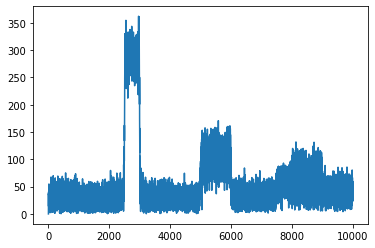
\includegraphics[scale=1]{fig/lab03/lab03_27_0.png}
		\caption{Спектр сигнала}
	\end{center}
\end{figure}

Видим, что гармоники накладываются друг на друга, и заметно что на частоте 2500 появляется возвышенность и на частоте около 5000 тоже. Это связано с тем, что в данном диапозоне равное изменение частоты занимает равное время.

\subsection{Упражнение 4}

В музыкальной терминологии «глиссандо» — это нота, которая скользит от одной высоты тона к другой, поэтому она похожа на чириканье. Найдите или сделайте запись глиссандо и постройте его спектрограмму.

Возьмём звук из репозитория учебника:

\begin{lstlisting}[language=Python]
if not os.path.exists('72475__rockwehrmann__glissup02.wav'):
    !wget https://github.com/AllenDowney/ThinkDSP/raw/master/code/72475__rockwehrmann__glissup02.wav
    

wave = read_wave('72475__rockwehrmann__glissup02.wav')

wave.make_spectrogram(512).plot(high=5000)
\end{lstlisting}
\begin{figure}[H]
	\begin{center}
		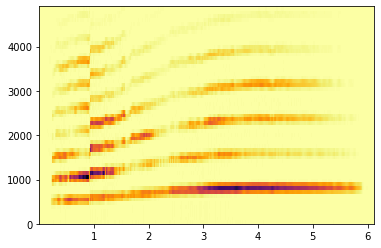
\includegraphics[scale=1]{fig/lab03/lab03_32_0.png}
		\caption{Спектрограмма сигнала}
	\end{center}
\end{figure}

Видим, что спектограмма очень похожа на наш чирп.

\subsection{Упражнение 5}

Тромбонист может играть глиссандо, выдвигая слайд тромбона и непрерывно дуя. По мере выдвижения ползуна общая длина трубки увеличивается, а результирующий шаг обратно пропорционален длине.
Предполагая, что игрок перемещает слайд с постоянной скоростью, как меняется ли частота со временем?

\noindent Напишите класс TromboneGliss, расширяющий класс Chirp и предоставляет evaluate. Создайте волну, имитирующую тромбон глиссандо от F3 вниз до C3 и обратно до F3. C3 — 262 Гц; F3 есть 349 Гц.

\begin{lstlisting}[language=Python]
class TromboneGliss(Chirp):

    
    def evaluate(self, ts):
        lengths = np.linspace(1.0 / self.start, 1.0 / self.end, len(ts))
        freqs = 1 / lengths
        dts = np.diff(ts, prepend=0)
        dphis = np.pi * 2 * freqs * dts
        phases = np.cumsum(dphis)
        ys = self.amp * np.cos(phases)
        return ys
\end{lstlisting}

Соединим сигналы:
\begin{lstlisting}[language=Python]
signal1 = TromboneGliss(262, 349)
wave1 = signal.make_wave(duration=1)

signal2 = TromboneGliss(349, 262)
wave2 = signal2.make_wave(duration=1)

result = wave1 | wave2
sp = result.make_spectrogram(1024)
sp.plot(high=1000)
\end{lstlisting}
\begin{figure}[H]
	\begin{center}
		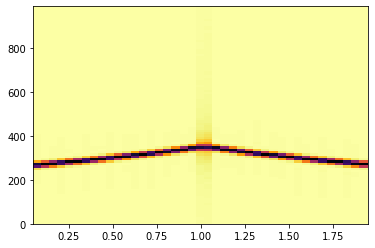
\includegraphics[scale=1]{fig/lab03/lab03_42_0.png}
		\caption{Спектрограмма сигнала}
	\end{center}
\end{figure}

Отчётливо слышно, как идут друг за другом 2 части.


\subsection{Упражнение 6}

Сделайте или найдите запись серии гласных звуков и посмотрите на спектрограмму. Сможете ли вы различить разные гласные?

Возьмём гласные из репозитория учебника:

\begin{lstlisting}[language=Python]
if not os.path.exists('87778__marcgascon7__vocals.wav'):
    !wget https://github.com/AllenDowney/ThinkDSP/raw/master/code/87778__marcgascon7__vocals.wav
wave = read_wave('87778__marcgascon7__vocals.wav')
wave.make_spectrogram(1024).plot(1000)
\end{lstlisting}
\begin{figure}[H]
	\begin{center}
		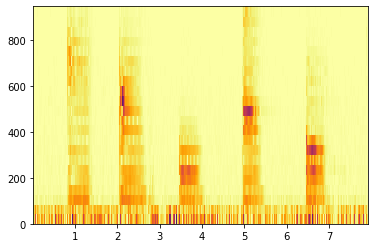
\includegraphics[scale=1]{fig/lab03/lab03_47_0.png}
		\caption{Спектрограмма гласных звуков}
	\end{center}
\end{figure}

На спектограмме видны пики, они и будут нашими гласными.

\subsection{Вывод}

В этой работе были расмотрены апериодические сигналы, частотные компоненты которых изменяются во времени. Также в этой главе были рассмотрены спектрограммы - способ визуализации апериодичных сигналов.